\PassOptionsToPackage{unicode=true}{hyperref} % options for packages loaded elsewhere
\PassOptionsToPackage{hyphens}{url}
%
\documentclass[]{book}
\usepackage{lmodern}
\usepackage{amssymb,amsmath}
\usepackage{ifxetex,ifluatex}
\usepackage{fixltx2e} % provides \textsubscript
\ifnum 0\ifxetex 1\fi\ifluatex 1\fi=0 % if pdftex
  \usepackage[T1]{fontenc}
  \usepackage[utf8]{inputenc}
  \usepackage{textcomp} % provides euro and other symbols
\else % if luatex or xelatex
  \usepackage{unicode-math}
  \defaultfontfeatures{Ligatures=TeX,Scale=MatchLowercase}
\fi
% use upquote if available, for straight quotes in verbatim environments
\IfFileExists{upquote.sty}{\usepackage{upquote}}{}
% use microtype if available
\IfFileExists{microtype.sty}{%
\usepackage[]{microtype}
\UseMicrotypeSet[protrusion]{basicmath} % disable protrusion for tt fonts
}{}
\IfFileExists{parskip.sty}{%
\usepackage{parskip}
}{% else
\setlength{\parindent}{0pt}
\setlength{\parskip}{6pt plus 2pt minus 1pt}
}
\usepackage{hyperref}
\hypersetup{
            pdftitle={Outstanding User Interfaces with Shiny},
            pdfauthor={David Granjon},
            pdfborder={0 0 0},
            breaklinks=true}
\urlstyle{same}  % don't use monospace font for urls
\usepackage{color}
\usepackage{fancyvrb}
\newcommand{\VerbBar}{|}
\newcommand{\VERB}{\Verb[commandchars=\\\{\}]}
\DefineVerbatimEnvironment{Highlighting}{Verbatim}{commandchars=\\\{\}}
% Add ',fontsize=\small' for more characters per line
\usepackage{framed}
\definecolor{shadecolor}{RGB}{248,248,248}
\newenvironment{Shaded}{\begin{snugshade}}{\end{snugshade}}
\newcommand{\AlertTok}[1]{\textcolor[rgb]{0.94,0.16,0.16}{#1}}
\newcommand{\AnnotationTok}[1]{\textcolor[rgb]{0.56,0.35,0.01}{\textbf{\textit{#1}}}}
\newcommand{\AttributeTok}[1]{\textcolor[rgb]{0.77,0.63,0.00}{#1}}
\newcommand{\BaseNTok}[1]{\textcolor[rgb]{0.00,0.00,0.81}{#1}}
\newcommand{\BuiltInTok}[1]{#1}
\newcommand{\CharTok}[1]{\textcolor[rgb]{0.31,0.60,0.02}{#1}}
\newcommand{\CommentTok}[1]{\textcolor[rgb]{0.56,0.35,0.01}{\textit{#1}}}
\newcommand{\CommentVarTok}[1]{\textcolor[rgb]{0.56,0.35,0.01}{\textbf{\textit{#1}}}}
\newcommand{\ConstantTok}[1]{\textcolor[rgb]{0.00,0.00,0.00}{#1}}
\newcommand{\ControlFlowTok}[1]{\textcolor[rgb]{0.13,0.29,0.53}{\textbf{#1}}}
\newcommand{\DataTypeTok}[1]{\textcolor[rgb]{0.13,0.29,0.53}{#1}}
\newcommand{\DecValTok}[1]{\textcolor[rgb]{0.00,0.00,0.81}{#1}}
\newcommand{\DocumentationTok}[1]{\textcolor[rgb]{0.56,0.35,0.01}{\textbf{\textit{#1}}}}
\newcommand{\ErrorTok}[1]{\textcolor[rgb]{0.64,0.00,0.00}{\textbf{#1}}}
\newcommand{\ExtensionTok}[1]{#1}
\newcommand{\FloatTok}[1]{\textcolor[rgb]{0.00,0.00,0.81}{#1}}
\newcommand{\FunctionTok}[1]{\textcolor[rgb]{0.00,0.00,0.00}{#1}}
\newcommand{\ImportTok}[1]{#1}
\newcommand{\InformationTok}[1]{\textcolor[rgb]{0.56,0.35,0.01}{\textbf{\textit{#1}}}}
\newcommand{\KeywordTok}[1]{\textcolor[rgb]{0.13,0.29,0.53}{\textbf{#1}}}
\newcommand{\NormalTok}[1]{#1}
\newcommand{\OperatorTok}[1]{\textcolor[rgb]{0.81,0.36,0.00}{\textbf{#1}}}
\newcommand{\OtherTok}[1]{\textcolor[rgb]{0.56,0.35,0.01}{#1}}
\newcommand{\PreprocessorTok}[1]{\textcolor[rgb]{0.56,0.35,0.01}{\textit{#1}}}
\newcommand{\RegionMarkerTok}[1]{#1}
\newcommand{\SpecialCharTok}[1]{\textcolor[rgb]{0.00,0.00,0.00}{#1}}
\newcommand{\SpecialStringTok}[1]{\textcolor[rgb]{0.31,0.60,0.02}{#1}}
\newcommand{\StringTok}[1]{\textcolor[rgb]{0.31,0.60,0.02}{#1}}
\newcommand{\VariableTok}[1]{\textcolor[rgb]{0.00,0.00,0.00}{#1}}
\newcommand{\VerbatimStringTok}[1]{\textcolor[rgb]{0.31,0.60,0.02}{#1}}
\newcommand{\WarningTok}[1]{\textcolor[rgb]{0.56,0.35,0.01}{\textbf{\textit{#1}}}}
\usepackage{longtable,booktabs}
% Fix footnotes in tables (requires footnote package)
\IfFileExists{footnote.sty}{\usepackage{footnote}\makesavenoteenv{longtable}}{}
\usepackage{graphicx,grffile}
\makeatletter
\def\maxwidth{\ifdim\Gin@nat@width>\linewidth\linewidth\else\Gin@nat@width\fi}
\def\maxheight{\ifdim\Gin@nat@height>\textheight\textheight\else\Gin@nat@height\fi}
\makeatother
% Scale images if necessary, so that they will not overflow the page
% margins by default, and it is still possible to overwrite the defaults
% using explicit options in \includegraphics[width, height, ...]{}
\setkeys{Gin}{width=\maxwidth,height=\maxheight,keepaspectratio}
\setlength{\emergencystretch}{3em}  % prevent overfull lines
\providecommand{\tightlist}{%
  \setlength{\itemsep}{0pt}\setlength{\parskip}{0pt}}
\setcounter{secnumdepth}{5}
% Redefines (sub)paragraphs to behave more like sections
\ifx\paragraph\undefined\else
\let\oldparagraph\paragraph
\renewcommand{\paragraph}[1]{\oldparagraph{#1}\mbox{}}
\fi
\ifx\subparagraph\undefined\else
\let\oldsubparagraph\subparagraph
\renewcommand{\subparagraph}[1]{\oldsubparagraph{#1}\mbox{}}
\fi

% set default figure placement to htbp
\makeatletter
\def\fps@figure{htbp}
\makeatother

\usepackage{booktabs}
\usepackage{amsthm}
\makeatletter
\def\thm@space@setup{%
  \thm@preskip=8pt plus 2pt minus 4pt
  \thm@postskip=\thm@preskip
}
\makeatother
\usepackage[]{natbib}
\bibliographystyle{apalike}

\title{Outstanding User Interfaces with Shiny}
\author{David Granjon}
\date{2020-04-13}

\begin{document}
\maketitle

{
\setcounter{tocdepth}{1}
\tableofcontents
}
\hypertarget{prerequisites}{%
\chapter*{Prerequisites}\label{prerequisites}}
\addcontentsline{toc}{chapter}{Prerequisites}

\begin{itemize}
\tightlist
\item
  Be familiar with \href{https://mastering-shiny.org}{Shiny}, the concept of modules
\item
  Basic knowledge in HTML and JavaScript is a plus but not mandatory.
\end{itemize}

\hypertarget{disclaimer}{%
\section*{Disclaimer}\label{disclaimer}}
\addcontentsline{toc}{section}{Disclaimer}

This book is not an HTML/Javascript/CSS course! It provides a \emph{survival kit} to be able to customize Shiny. I am sure however that readers will want to explore more about these topics.

\hypertarget{is-this-book-for-me}{%
\section*{Is this book for me?}\label{is-this-book-for-me}}
\addcontentsline{toc}{section}{Is this book for me?}

You should read this book if you answer yes to at least 2 of the following questions:

\begin{itemize}
\tightlist
\item
  Do you want to know how to develop outstanding shiny apps?
\item
  Have you ever wondered how to develop new input widgets?
\end{itemize}

\hypertarget{related-content}{%
\section*{Related content}\label{related-content}}
\addcontentsline{toc}{section}{Related content}

See the \href{https://rstudio.cloud}{RStudio Cloud} dedicated project.

\hypertarget{intro}{%
\chapter{Introduction}\label{intro}}

In the past two years, there were various Shiny focused resources introducing basic as well as advanced topics such as modules and Javascript/R interactions. However, handling advanced user interfaces was never an emphasis. Clients often desire custom designs, yet this generally exceeds core features of Shiny. We recognized that R App developers lacking a significant background in web development may have found this requirement to be overwhelming. Consequently, the aim of this book is to provide readers the necessary knowledge to extend Shiny's layout, input widgets and output elements. Thi book is organized into four parts. We first go through the basics of HTML, JavaScript and jQuery. In part 2, we dive into the \{htmltools\} package, providing functions to create and manipulate shiny tags as well as manage dependencies. Part 3 homes in on the development of a new template on top of Shiny by demonstrating examples from the \{bs4Dash\} and \{shinyMobile\} packages, part of the RinteRface project.

\hypertarget{part-survival-kit}{%
\part*{Survival Kit}\label{part-survival-kit}}
\addcontentsline{toc}{part}{Survival Kit}

This part will give you basis in HTML, JavaScript to get started\ldots{}

\hypertarget{survival-kit-html}{%
\chapter{HTML}\label{survival-kit-html}}

\hypertarget{survival-kit-javascript}{%
\chapter{JavaScript}\label{survival-kit-javascript}}

\hypertarget{survival-kit-shiny}{%
\chapter{Shiny}\label{survival-kit-shiny}}

\hypertarget{part-htmltools}{%
\part*{htmltools}\label{part-htmltools}}
\addcontentsline{toc}{part}{htmltools}

While building a custom html template, you will need to know more about the wonderful \href{https://github.com/rstudio/htmltools}{htmltools} developed by Winston Chang, member of the shiny core team. It has the same spirit as devtools, that is, making your web developer life easier. What follows does not have the pretention to be an exhaustive guide about this package. Yet, it will provide you yith the main tools to be more efficient.

\hypertarget{htmltools-overview}{%
\chapter{htmltools overview}\label{htmltools-overview}}

\hypertarget{html-tags}{%
\section{HTML Tags}\label{html-tags}}

htmltools contains tools to write HTML tags we saw in Chapter \ref{survival-kit-html}. Within your package code, your tags will be like:

\begin{Shaded}
\begin{Highlighting}[]
\CommentTok{# we use htmltools tags instead of shiny}
\NormalTok{htmltools}\OperatorTok{::}\NormalTok{tags}\OperatorTok{$}\KeywordTok{div}\NormalTok{(...)}
\end{Highlighting}
\end{Shaded}

If you had to gather multiple tags together, prefer \texttt{tagList()} as \texttt{list()}, although the HTML output is the same. The first has the shiny.tag.list class in addition to list. (The \href{http://golemverse.org}{Golem} package allows to test if a R object is a tag list, therefore using list would make the test fail).

\hypertarget{notations}{%
\section{Notations}\label{notations}}

Whether to use \texttt{tags\$div} or \texttt{div} depends if the tag is exported by default.
For instance, you could use \texttt{htmltools::div} but not \texttt{htmltools::nav} since nav does not have a dedicated function (only for p, h1, h2, h3, h4, h5, h6, a, br, div, span, pre, code, img, strong, em, hr).
Rather use \texttt{htmltools::tags\$nav}. Alternatively, there exists a function (in shiny and htmltools)
called \texttt{withTags()}. Wrapping your code in this function enables you to use \texttt{withTags(nav(),\ ...)}
instead of \texttt{tags\$nav()}.

\hypertarget{adding-new-tags}{%
\section{Adding new tags}\label{adding-new-tags}}

The \texttt{tag} function allows to add extra HTML tags not already defined. You may use it as follows:

\begin{Shaded}
\begin{Highlighting}[]
\KeywordTok{tag}\NormalTok{(}\StringTok{"test"}\NormalTok{, }\KeywordTok{list}\NormalTok{(}\DataTypeTok{class =} \StringTok{"test"}\NormalTok{, }\KeywordTok{p}\NormalTok{(}\StringTok{"Custom Tag"}\NormalTok{)))}
\CommentTok{# structure below}
\NormalTok{█─tag }
\NormalTok{├─}\StringTok{"test"} 
\NormalTok{└─█─list }
\NormalTok{  ├─class =}\StringTok{ "test"} 
\NormalTok{  └─█─p }
\NormalTok{    └─}\StringTok{"Custom Tag"} 
\end{Highlighting}
\end{Shaded}

\hypertarget{alternative-way-to-write-tags}{%
\section{Alternative way to write tags}\label{alternative-way-to-write-tags}}

htmltools comes with the \texttt{HTML()} function that you can feed with raw HTML:

\begin{Shaded}
\begin{Highlighting}[]
\KeywordTok{HTML}\NormalTok{(}\StringTok{'<div>Blabla</div>'}\NormalTok{)}
\CommentTok{# will render exactly like}
\KeywordTok{div}\NormalTok{(}\StringTok{"Blabla"}\NormalTok{)}

\CommentTok{# but there class is different}
\KeywordTok{class}\NormalTok{(}\KeywordTok{HTML}\NormalTok{(}\StringTok{'<div>Blabla</div>'}\NormalTok{))}
\KeywordTok{class}\NormalTok{(}\KeywordTok{div}\NormalTok{(}\StringTok{"Blabla"}\NormalTok{))}
\end{Highlighting}
\end{Shaded}

You will not be able to use tag related functions, as in the following parts.
Therefore, I strongly recommand using R and not mixing HTML in R. Interestingly, if
you want to convert HTML to R code, there is a Shiny App developed by Alan
Dipert from RStudio, namely \href{https://github.com/alandipert/html2r}{html2R}. There
are some issues, non standard attributes (like \texttt{data-toggle}) are not correctly processed but there are \href{https://github.com/alandipert/html2r/issues/2}{fixes}. This will save you precious time!

\href{https://alandipert.shinyapps.io/html2r/}{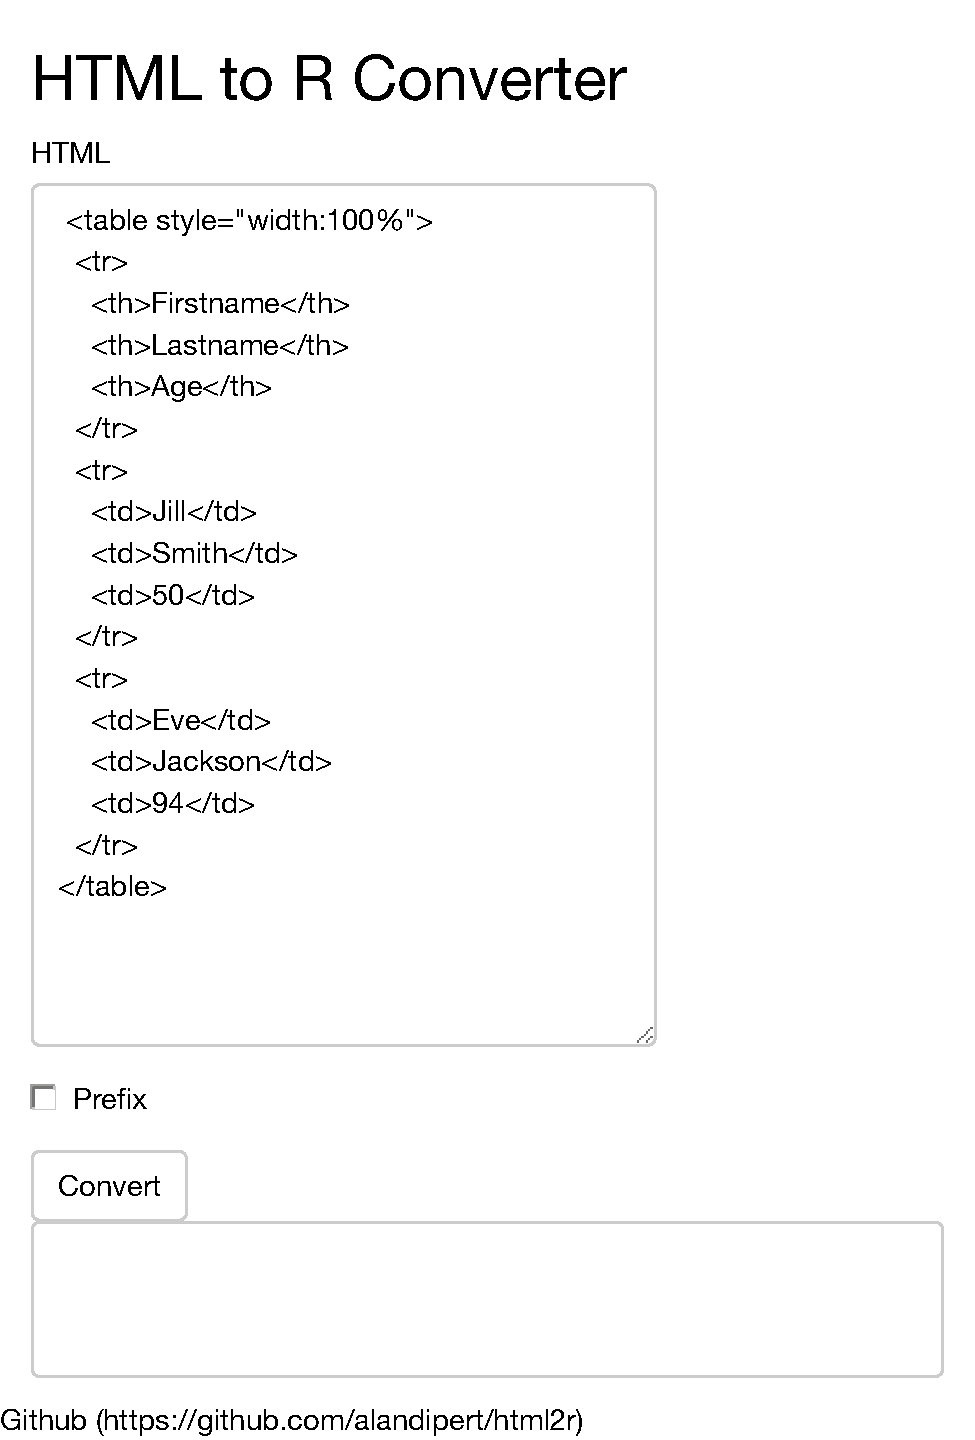
\includegraphics{outstanding-shiny-ui_files/figure-latex/unnamed-chunk-5-1.pdf}}

\hypertarget{playing-with-tags}{%
\section{Playing with tags}\label{playing-with-tags}}

\hypertarget{tags-structure}{%
\subsection{Tags structure}\label{tags-structure}}

According to the \texttt{tag} function, a tag has:

\begin{itemize}
\tightlist
\item
  a name such as span, div, h1 \ldots{} \texttt{tag\$name}
\item
  some attributes, which you can access with \texttt{tag\$attribs}
\item
  children, which you can access with \texttt{tag\$children}
\item
  a class, namely ``shiny.tag''
\end{itemize}

For instance:

\begin{Shaded}
\begin{Highlighting}[]
\CommentTok{# create the tag}
\NormalTok{myTag <-}\StringTok{ }\KeywordTok{div}\NormalTok{(}
  \DataTypeTok{class =} \StringTok{"divclass"}\NormalTok{, }
  \DataTypeTok{id =} \StringTok{"first"}\NormalTok{,}
  \KeywordTok{h1}\NormalTok{(}\StringTok{"Here comes your baby"}\NormalTok{),}
  \KeywordTok{span}\NormalTok{(}\DataTypeTok{class =} \StringTok{"child"}\NormalTok{, }\DataTypeTok{id =} \StringTok{"baby"}\NormalTok{, }\StringTok{"Crying"}\NormalTok{)}
\NormalTok{)}
\CommentTok{# access its name}
\NormalTok{myTag}\OperatorTok{$}\NormalTok{name}
\CommentTok{# access its attributes (id and class)}
\NormalTok{myTag}\OperatorTok{$}\NormalTok{attribs}
\CommentTok{# access children (returns a list of 2 elements)}
\NormalTok{myTag}\OperatorTok{$}\NormalTok{children}
\CommentTok{# access its class}
\KeywordTok{class}\NormalTok{(myTag)}
\end{Highlighting}
\end{Shaded}

How to modify the class of the second child, namely span?

\begin{Shaded}
\begin{Highlighting}[]
\NormalTok{second_children <-}\StringTok{ }\NormalTok{myTag}\OperatorTok{$}\NormalTok{children[[}\DecValTok{2}\NormalTok{]]}
\NormalTok{second_children}\OperatorTok{$}\NormalTok{attribs}\OperatorTok{$}\NormalTok{class <-}\StringTok{ "adult"}
\NormalTok{myTag}
\CommentTok{# Hummm, this is not working ...}
\end{Highlighting}
\end{Shaded}

Why is this not working? By assigning \texttt{myTag\$children{[}{[}2{]}{]}} to second\_children, \texttt{second\_children\$attribs\$class\ \textless{}-\ "adult"} modifies the class of the copy and not the original object. Thus we do:

\begin{Shaded}
\begin{Highlighting}[]
\NormalTok{myTag}\OperatorTok{$}\NormalTok{children[[}\DecValTok{2}\NormalTok{]]}\OperatorTok{$}\NormalTok{attribs}\OperatorTok{$}\NormalTok{class <-}\StringTok{ "adult"}
\NormalTok{myTag}
\end{Highlighting}
\end{Shaded}

In the following section we explore helper functions, such as \texttt{tagAppendChild} from htmltools.

\hypertarget{useful-functions-for-tags}{%
\subsection{Useful functions for tags}\label{useful-functions-for-tags}}

htmltools and Shiny have powerful functions to easily add attributes to tags, check for existing attributes, get attributes and add other siblings to a list of tags.

\hypertarget{add-attributes}{%
\subsubsection{Add attributes}\label{add-attributes}}

\begin{itemize}
\tightlist
\item
  \texttt{tagAppendAttributes}: this function allow you to add a new attribute to the current tag.
\end{itemize}

For instance, assuming you created a div for which you forgot to add an id attribute:

\begin{Shaded}
\begin{Highlighting}[]
\NormalTok{mydiv <-}\StringTok{ }\KeywordTok{div}\NormalTok{(}\StringTok{"Where is my brain"}\NormalTok{)}
\NormalTok{mydiv <-}\StringTok{ }\KeywordTok{tagAppendAttributes}\NormalTok{(mydiv, }\DataTypeTok{id =} \StringTok{"here_it_is"}\NormalTok{)}
\end{Highlighting}
\end{Shaded}

You can pass as many attributes as you want, including non standard attributes such as \texttt{data-toggle} (see Bootstrap 3 tabs for instance):

\begin{Shaded}
\begin{Highlighting}[]
\NormalTok{mydiv <-}\StringTok{ }\KeywordTok{tagAppendAttributes}\NormalTok{(mydiv, }\StringTok{`}\DataTypeTok{data-toggle}\StringTok{`}\NormalTok{ =}\StringTok{ "tabs"}\NormalTok{)}
\CommentTok{# even though you could proceed as follows}
\NormalTok{mydiv}\OperatorTok{$}\NormalTok{attribs[[}\StringTok{"aria-controls"}\NormalTok{]] <-}\StringTok{ "home"}
\end{Highlighting}
\end{Shaded}

\hypertarget{check-if-tag-has-specific-attribute}{%
\subsubsection{Check if tag has specific attribute}\label{check-if-tag-has-specific-attribute}}

\begin{itemize}
\tightlist
\item
  \texttt{tagHasAttribute}: to check if a tag has a specific attribute
\end{itemize}

\begin{Shaded}
\begin{Highlighting}[]
\CommentTok{# I want to know if div has a class}
\NormalTok{mydiv <-}\StringTok{ }\KeywordTok{div}\NormalTok{(}\DataTypeTok{class =} \StringTok{"myclass"}\NormalTok{)}
\NormalTok{has_class <-}\StringTok{ }\KeywordTok{tagHasAttribute}\NormalTok{(mydiv, }\StringTok{"class"}\NormalTok{)}
\NormalTok{has_class}
\CommentTok{# if you are familiar with %>%}
\NormalTok{has_class <-}\StringTok{ }\NormalTok{mydiv }\OperatorTok\StringTok{ }\KeywordTok{tagHasAttribute}\NormalTok{(}\StringTok{"class"}\NormalTok{)}
\NormalTok{has_class}
\end{Highlighting}
\end{Shaded}

\hypertarget{get-all-attributes}{%
\subsubsection{Get all attributes}\label{get-all-attributes}}

\begin{itemize}
\tightlist
\item
  \texttt{tagGetAttribute}: to get the value of the targeted attributes, if it exists, otherwise NULL.
\end{itemize}

\begin{Shaded}
\begin{Highlighting}[]
\NormalTok{mydiv <-}\StringTok{ }\KeywordTok{div}\NormalTok{(}\DataTypeTok{class =} \StringTok{"test"}\NormalTok{)}
\CommentTok{# returns the class}
\KeywordTok{tagGetAttribute}\NormalTok{(mydiv, }\StringTok{"class"}\NormalTok{)}
\CommentTok{# returns NULL}
\KeywordTok{tagGetAttribute}\NormalTok{(mydiv, }\StringTok{"id"}\NormalTok{)}
\end{Highlighting}
\end{Shaded}

\hypertarget{set-childchildren}{%
\subsubsection{Set child/children}\label{set-childchildren}}

\begin{itemize}
\tightlist
\item
  \texttt{tagSetChildren} allows to create children for a given tag. For instance:
\end{itemize}

\begin{Shaded}
\begin{Highlighting}[]
\NormalTok{mydiv <-}\StringTok{ }\KeywordTok{div}\NormalTok{(}\DataTypeTok{class =} \StringTok{"parent"}\NormalTok{, }\DataTypeTok{id =} \StringTok{"mother"}\NormalTok{, }\StringTok{"Not the mama!!!"}\NormalTok{)}
\CommentTok{# mydiv has 1 child "Not the mama!!!"}
\NormalTok{mydiv }
\NormalTok{children <-}\StringTok{ }\KeywordTok{lapply}\NormalTok{(}\DecValTok{1}\OperatorTok{:}\DecValTok{3}\NormalTok{, span)}
\NormalTok{mydiv <-}\StringTok{ }\KeywordTok{tagSetChildren}\NormalTok{(mydiv, children)}
\CommentTok{# mydiv has 3 children, the first one was removed}
\NormalTok{mydiv }
\end{Highlighting}
\end{Shaded}

Notice that \texttt{tagSetChildren} removes all existing children. Below we see another set of functions to add children while conserving existing ones.

\hypertarget{add-child-or-children}{%
\subsubsection{Add child or children}\label{add-child-or-children}}

\begin{itemize}
\tightlist
\item
  \texttt{tagAppendChild} and \texttt{tagAppendChildren}: add other tags to an existing tag.
  Whereas \texttt{tagAppendChild} only takes one tag, you can pass a list of tags to \texttt{tagAppendChildren}.
\end{itemize}

\begin{Shaded}
\begin{Highlighting}[]
\NormalTok{mydiv <-}\StringTok{ }\KeywordTok{div}\NormalTok{(}\DataTypeTok{class =} \StringTok{"parent"}\NormalTok{, }\DataTypeTok{id =} \StringTok{"mother"}\NormalTok{, }\StringTok{"Not the mama!!!"}\NormalTok{)}
\NormalTok{otherTag <-}\StringTok{ }\KeywordTok{span}\NormalTok{(}\StringTok{"I am your child"}\NormalTok{)}
\NormalTok{mydiv <-}\StringTok{ }\KeywordTok{tagAppendChild}\NormalTok{(mydiv, otherTag)}
\end{Highlighting}
\end{Shaded}

You might wonder why there is no \texttt{tagRemoveChild} or \texttt{tagRemoveAttributes}.
Let's look at the \texttt{tagAppendChild}

\begin{Shaded}
\begin{Highlighting}[]
\NormalTok{tagAppendChild <-}\StringTok{ }\ControlFlowTok{function}\NormalTok{ (tag, child) \{}
\NormalTok{  tag}\OperatorTok{$}\NormalTok{children[[}\KeywordTok{length}\NormalTok{(tag}\OperatorTok{$}\NormalTok{children) }\OperatorTok{+}\StringTok{ }\DecValTok{1}\NormalTok{]] <-}\StringTok{ }\NormalTok{child}
\NormalTok{  tag}
\NormalTok{\}}
\end{Highlighting}
\end{Shaded}

Below we write the \texttt{tagRemoveChild}, where tag is the target and n is the position to remove in the list of children:

\begin{Shaded}
\begin{Highlighting}[]
\NormalTok{mydiv <-}\StringTok{ }\KeywordTok{div}\NormalTok{(}\DataTypeTok{class =} \StringTok{"parent"}\NormalTok{, }\DataTypeTok{id =} \StringTok{"mother"}\NormalTok{, }\StringTok{"Not the mama!!!"}\NormalTok{, }\KeywordTok{span}\NormalTok{(}\StringTok{"Hey!"}\NormalTok{))}

\CommentTok{# we create the tagRemoveChild function}
\NormalTok{tagRemoveChild <-}\StringTok{ }\ControlFlowTok{function}\NormalTok{(tag, n) \{}
  \CommentTok{# check if the list is empty}
  \ControlFlowTok{if}\NormalTok{ (rlang}\OperatorTok{::}\KeywordTok{is_empty}\NormalTok{(tag}\OperatorTok{$}\NormalTok{children)) \{}
    \KeywordTok{stop}\NormalTok{(}\KeywordTok{paste}\NormalTok{(tag}\OperatorTok{$}\NormalTok{name, }\StringTok{"does not have any children"}\NormalTok{))}
\NormalTok{  \}}
\NormalTok{  tag}\OperatorTok{$}\NormalTok{children[n] <-}\StringTok{ }\OtherTok{NULL}
\NormalTok{  tag}
\NormalTok{\}}
\NormalTok{mydiv <-}\StringTok{ }\KeywordTok{tagRemoveChild}\NormalTok{(mydiv, }\DecValTok{1}\NormalTok{)}
\NormalTok{mydiv}
\end{Highlighting}
\end{Shaded}

When defining the \texttt{tagRemoveChild}, we choose \texttt{{[}} instead of \texttt{{[}{[}} to allow to select multiple list elements:

\begin{Shaded}
\begin{Highlighting}[]
\NormalTok{mydiv <-}\StringTok{ }\KeywordTok{div}\NormalTok{(}\DataTypeTok{class =} \StringTok{"parent"}\NormalTok{, }\DataTypeTok{id =} \StringTok{"mother"}\NormalTok{, }\StringTok{"Not the mama!!!"}\NormalTok{, }\StringTok{"Hey!"}\NormalTok{)}
\CommentTok{# fails}
\StringTok{`}\DataTypeTok{[[}\StringTok{`}\NormalTok{(mydiv}\OperatorTok{$}\NormalTok{children, }\KeywordTok{c}\NormalTok{(}\DecValTok{1}\NormalTok{, }\DecValTok{2}\NormalTok{))}
\CommentTok{# works}
\StringTok{`}\DataTypeTok{[}\StringTok{`}\NormalTok{(mydiv}\OperatorTok{$}\NormalTok{children, }\KeywordTok{c}\NormalTok{(}\DecValTok{1}\NormalTok{, }\DecValTok{2}\NormalTok{))}
\end{Highlighting}
\end{Shaded}

Alternatively, we could also create a \texttt{tagRemoveChildren} function. Also notice that the function raises an error if the provided tag does not have children.

\hypertarget{other-interesting-functions}{%
\subsection{Other interesting functions}\label{other-interesting-functions}}

The \href{https://github.com/ThinkR-open/brighter}{brighter} package written by Colin Fay contains neat functions to edit your tags. Particularly, the \texttt{tagRemoveAttributes}

\begin{Shaded}
\begin{Highlighting}[]
\NormalTok{remotes}\OperatorTok{::}\KeywordTok{install_github}\NormalTok{(}\StringTok{"Thinkr-open/brighter"}\NormalTok{)}
\KeywordTok{library}\NormalTok{(brighter)}
\end{Highlighting}
\end{Shaded}

\begin{Shaded}
\begin{Highlighting}[]
\NormalTok{mydiv <-}\StringTok{ }\KeywordTok{div}\NormalTok{(}\DataTypeTok{class =} \StringTok{"test"}\NormalTok{, }\DataTypeTok{id =} \StringTok{"coucou"}\NormalTok{, }\StringTok{"Hello"}\NormalTok{)}
\KeywordTok{tagRemoveAttributes}\NormalTok{(mydiv, }\StringTok{"class"}\NormalTok{, }\StringTok{"id"}\NormalTok{)}
\end{Highlighting}
\end{Shaded}

\hypertarget{htmltools-dependencies}{%
\chapter{Dependency utilities}\label{htmltools-dependencies}}

When creating a new template, you sometimes need to import custom HTML dependencies
that do not come along with shiny. No problem, htmltools is here for you (shiny also
contains these functions).

\begin{Shaded}
\begin{Highlighting}[]
\KeywordTok{library}\NormalTok{(shiny)}
\KeywordTok{library}\NormalTok{(shinydashboard)}
\end{Highlighting}
\end{Shaded}

\hypertarget{the-dirty-approach}{%
\section{The dirty approach}\label{the-dirty-approach}}

Let's consider the following example. I want to include a bootstrap 4 card in a shiny app.
This example is taken from an interesting question \href{https://community.rstudio.com/t/create-a-div-using-htmltools-withtags/22439/2}{here}.
The naive approach would be to include the HTML code directly in the app code

\begin{Shaded}
\begin{Highlighting}[]
\CommentTok{# we create the card function before}
\NormalTok{my_card <-}\StringTok{ }\ControlFlowTok{function}\NormalTok{(...) \{}
\NormalTok{  htmltools}\OperatorTok{::}\KeywordTok{withTags}\NormalTok{(}
    \KeywordTok{div}\NormalTok{(}
      \DataTypeTok{class =} \StringTok{"card border-success mb-3"}\NormalTok{,}
      \KeywordTok{div}\NormalTok{(}\DataTypeTok{class =} \StringTok{"card-header bg-transparent border-success"}\NormalTok{),}
      \KeywordTok{div}\NormalTok{(}
        \DataTypeTok{class =} \StringTok{"card-body text-success"}\NormalTok{,}
        \KeywordTok{h3}\NormalTok{(}\DataTypeTok{class =} \StringTok{"card-title"}\NormalTok{, }\StringTok{"title"}\NormalTok{),}
        \KeywordTok{p}\NormalTok{(}\DataTypeTok{class =} \StringTok{"card-text"}\NormalTok{, ...)}
\NormalTok{      ),}
      \KeywordTok{div}\NormalTok{(}\DataTypeTok{class =} \StringTok{"card-footer bg-transparent border-success"}\NormalTok{, }\StringTok{"footer"}\NormalTok{)}
\NormalTok{    )}
\NormalTok{  )}
\NormalTok{\}}

\CommentTok{# we build our app}
\KeywordTok{shinyApp}\NormalTok{(}
  \DataTypeTok{ui =} \KeywordTok{fluidPage}\NormalTok{(}
    \KeywordTok{fluidRow}\NormalTok{(}
      \KeywordTok{column}\NormalTok{(}
        \DataTypeTok{width =} \DecValTok{6}\NormalTok{,}
        \DataTypeTok{align =} \StringTok{"center"}\NormalTok{,}
        \KeywordTok{br}\NormalTok{(),}
        \KeywordTok{my_card}\NormalTok{(}\StringTok{"blablabla. PouetPouet Pouet."}\NormalTok{)}
\NormalTok{      )}
\NormalTok{    )}
\NormalTok{  ),}
  \DataTypeTok{server =} \ControlFlowTok{function}\NormalTok{(input, output) \{\}}
\NormalTok{)}
\end{Highlighting}
\end{Shaded}

and desesperately see that nothing is displayed. If you remember, this was expected since
shiny does not contain bootstrap 4 dependencies and this card is unfortunately a
bootstrap 4 object. Don't panic! We just need to tell shiny to load the css we need to display
this card (if required, we could include the javascript as well). We could use either
\texttt{includeCSS()}, \texttt{tags\$head(tags\$link(rel\ =\ "stylesheet",\ type\ =\ "text/css",\ href\ =\ "custom.css"))}. See
more \href{https://shiny.rstudio.com/articles/css.html}{here}.

\begin{Shaded}
\begin{Highlighting}[]
\KeywordTok{shinyApp}\NormalTok{(}
  \DataTypeTok{ui =} \KeywordTok{fluidPage}\NormalTok{(}
    \CommentTok{# load the css code}
    \KeywordTok{includeCSS}\NormalTok{(}\DataTypeTok{path =} \StringTok{"https://maxcdn.bootstrapcdn.com/bootstrap/4.0.0/css/bootstrap.min.css"}\NormalTok{),}
    \KeywordTok{fluidRow}\NormalTok{(}
      \KeywordTok{column}\NormalTok{(}
        \DataTypeTok{width =} \DecValTok{6}\NormalTok{,}
        \DataTypeTok{align =} \StringTok{"center"}\NormalTok{,}
        \KeywordTok{br}\NormalTok{(),}
        \KeywordTok{my_card}\NormalTok{(}\StringTok{"blablabla. PouetPouet Pouet."}\NormalTok{)}
\NormalTok{      )}
\NormalTok{    )}
\NormalTok{  ),}
  \DataTypeTok{server =} \ControlFlowTok{function}\NormalTok{(input, output) \{\}}
\NormalTok{)}
\end{Highlighting}
\end{Shaded}

The card is ugly (which is another problem we will fix later) but at least displayed.

When I say this approach is dirty, it is because it will not be easily re-usable by others.
Instead, we prefer a packaging approach, like in the next section.

\hypertarget{the-clean-approach}{%
\section{The clean approach}\label{the-clean-approach}}

We will use the \texttt{htmlDependency} and \texttt{attachDependencies} functions from htmltools.
The htmlDependency takes several arguments:

\begin{itemize}
\tightlist
\item
  the name of your dependency
\item
  the version (useful to remember on which version it is built upon)
\item
  a path to the dependency (can be a CDN or a local folder)
\item
  script and stylesheet to respectively pass css and scripts
\end{itemize}

\begin{Shaded}
\begin{Highlighting}[]
\CommentTok{# handle dependency}
\NormalTok{card_css <-}\StringTok{ "bootstrap.min.css"}
\NormalTok{bs4_card_dep <-}\StringTok{ }\ControlFlowTok{function}\NormalTok{() \{}
\NormalTok{  htmltools}\OperatorTok{::}\KeywordTok{htmlDependency}\NormalTok{(}
    \DataTypeTok{name =} \StringTok{"bs4_card"}\NormalTok{,}
    \DataTypeTok{version =} \StringTok{"1.0"}\NormalTok{,}
    \DataTypeTok{src =} \KeywordTok{c}\NormalTok{(}\DataTypeTok{href =} \StringTok{"https://maxcdn.bootstrapcdn.com/bootstrap/4.0.0/css/"}\NormalTok{),}
    \DataTypeTok{stylesheet =}\NormalTok{ card_css}
\NormalTok{  )}
\NormalTok{\}}
\end{Highlighting}
\end{Shaded}

We create the card tag and give it the bootstrap 4 dependency through the \texttt{attachDependencies()}
function.

\begin{Shaded}
\begin{Highlighting}[]
\CommentTok{# create the card}
\NormalTok{my_card <-}\StringTok{ }\ControlFlowTok{function}\NormalTok{(...) \{}
\NormalTok{  cardTag <-}\StringTok{ }\NormalTok{htmltools}\OperatorTok{::}\KeywordTok{withTags}\NormalTok{(}
    \KeywordTok{div}\NormalTok{(}
      \DataTypeTok{class =} \StringTok{"card border-success mb-3"}\NormalTok{,}
      \KeywordTok{div}\NormalTok{(}\DataTypeTok{class =} \StringTok{"card-header bg-transparent border-success"}\NormalTok{),}
      \KeywordTok{div}\NormalTok{(}
        \DataTypeTok{class =} \StringTok{"card-body text-success"}\NormalTok{,}
        \KeywordTok{h3}\NormalTok{(}\DataTypeTok{class =} \StringTok{"card-title"}\NormalTok{, }\StringTok{"title"}\NormalTok{),}
        \KeywordTok{p}\NormalTok{(}\DataTypeTok{class =} \StringTok{"card-text"}\NormalTok{, ...)}
\NormalTok{      ),}
      \KeywordTok{div}\NormalTok{(}\DataTypeTok{class =} \StringTok{"card-footer bg-transparent border-success"}\NormalTok{, }\StringTok{"footer"}\NormalTok{)}
\NormalTok{    )}
\NormalTok{  )}
  
  \CommentTok{# attach dependencies}
\NormalTok{  htmltools}\OperatorTok{::}\KeywordTok{attachDependencies}\NormalTok{(cardTag, }\KeywordTok{bs4_card_dep}\NormalTok{())}
  
\NormalTok{\}}
\end{Highlighting}
\end{Shaded}

We finally run our app:

\begin{Shaded}
\begin{Highlighting}[]
\CommentTok{# run shiny app }
\NormalTok{ui <-}\StringTok{ }\KeywordTok{fluidPage}\NormalTok{(}
  \DataTypeTok{title =} \StringTok{"Hello Shiny!"}\NormalTok{,}
  \KeywordTok{fluidRow}\NormalTok{(}
    \KeywordTok{column}\NormalTok{(}
      \DataTypeTok{width =} \DecValTok{6}\NormalTok{,}
      \DataTypeTok{align =} \StringTok{"center"}\NormalTok{,}
      \KeywordTok{br}\NormalTok{(),}
      \KeywordTok{my_card}\NormalTok{(}\StringTok{"blablabla. PouetPouet Pouet."}\NormalTok{)}
\NormalTok{    )}
\NormalTok{  )}
\NormalTok{)}

\KeywordTok{shinyApp}\NormalTok{(ui, }\DataTypeTok{server =} \ControlFlowTok{function}\NormalTok{(input, output) \{ \})}
\end{Highlighting}
\end{Shaded}

With this approach, you could develop a package of custom dependencies that people
could use when they need to add custom elements in shiny.

\hypertarget{another-example-importing-html-dependencies-from-other-packages}{%
\section{Another example: Importing HTML dependencies from other packages}\label{another-example-importing-html-dependencies-from-other-packages}}

You may know shinydashboard, a package to design dashboards with shiny. In the following, we would like to integrate the box component in a classic Shiny App (without the dashboard layout). However, if you try to include the Shinydashboard box tag, you will notice that nothing is displayed since Shiny does not have shinydashboard dependencies. Fortunately htmltools contains a function, namely \texttt{findDependencies} that looks for all dependencies attached to a tag. How about extracting shinydashboard dependencies? Before going futher, let's define the basic skeleton of a shinydashboard:

\begin{Shaded}
\begin{Highlighting}[]
\KeywordTok{shinyApp}\NormalTok{(}
  \DataTypeTok{ui =} \KeywordTok{dashboardPage}\NormalTok{(}
    \KeywordTok{dashboardHeader}\NormalTok{(),}
    \KeywordTok{dashboardSidebar}\NormalTok{(),}
    \KeywordTok{dashboardBody}\NormalTok{(),}
    \DataTypeTok{title =} \StringTok{"Dashboard example"}
\NormalTok{  ),}
  \DataTypeTok{server =} \ControlFlowTok{function}\NormalTok{(input, output) \{ \}}
\NormalTok{)}
\end{Highlighting}
\end{Shaded}

We don't need to understand shinydashboard details. However, if you are interested to dig in, \href{https://rstudio.github.io/shinydashboard/}{help yourself}. What is important here is the main
wrapper function \texttt{dashboardPage}. (You should already be familiar with \texttt{fluidPage}, another wrapper function). We apply \texttt{findDependencies} on \texttt{dashboardPage}.

\begin{Shaded}
\begin{Highlighting}[]
\NormalTok{deps <-}\StringTok{ }\KeywordTok{findDependencies}\NormalTok{(}
\NormalTok{  shinydashboard}\OperatorTok{::}\KeywordTok{dashboardPage}\NormalTok{(}
    \DataTypeTok{header =}\NormalTok{ shinydashboard}\OperatorTok{::}\KeywordTok{dashboardHeader}\NormalTok{(), }
    \DataTypeTok{sidebar =}\NormalTok{ shinydashboard}\OperatorTok{::}\KeywordTok{dashboardSidebar}\NormalTok{(), }
    \DataTypeTok{body =}\NormalTok{ shinydashboard}\OperatorTok{::}\KeywordTok{dashboardBody}\NormalTok{()}
\NormalTok{  )}
\NormalTok{)}
\NormalTok{deps}
\end{Highlighting}
\end{Shaded}

deps is a list containg 4 dependencies:

\begin{itemize}
\tightlist
\item
  \href{https://fontawesome.com}{Font Awesome} handles icons
\item
  \href{https://getbootstrap.com/docs/3.3/}{Bootstrap} is the main HTML/CSS/JS template. Importantly,
  please note the version 3.3.7, whereas the current is 4.3.1
\item
  \href{https://adminlte.io}{AdminLTE} is the dependency containg HTML/CSS/JS related to the admin template.
  It is closely linked to Bootstrap 3.
\item
  shinydashboard, the CSS and javascript necessary for shinydashboard to work properly. In practice,
  integrating custom HTML templates to shiny does not usually work out of the box for many reasons (Explain why!) and some modifications are necessary.
\end{itemize}

\begin{verbatim}
[[1]]
List of 10
$ name      : chr "font-awesome"
$ version   : chr "5.3.1"
$ src       :List of 1
..$ file: chr "www/shared/fontawesome"
$ meta      : NULL
$ script    : NULL
$ stylesheet: chr [1:2] "css/all.min.css" "css/v4-shims.min.css"
$ head      : NULL
$ attachment: NULL
$ package   : chr "shiny"
$ all_files : logi TRUE
- attr(*, "class")= chr "html_dependency"
[[2]]
List of 10
$ name      : chr "bootstrap"
$ version   : chr "3.3.7"
$ src       :List of 2
..$ href: chr "shared/bootstrap"
..$ file: chr "/Library/Frameworks/R.framework/Versions/3.5/Resources/library/shiny/www/shared/bootstrap"
$ meta      :List of 1
..$ viewport: chr "width=device-width, initial-scale=1"
$ script    : chr [1:3] "js/bootstrap.min.js" "shim/html5shiv.min.js" "shim/respond.min.js"
$ stylesheet: chr "css/bootstrap.min.css"
$ head      : NULL
$ attachment: NULL
$ package   : NULL
$ all_files : logi TRUE
- attr(*, "class")= chr "html_dependency"
[[3]]
List of 10
$ name      : chr "AdminLTE"
$ version   : chr "2.0.6"
$ src       :List of 1
..$ file: chr "/Library/Frameworks/R.framework/Versions/3.5/Resources/library/shinydashboard/AdminLTE"
$ meta      : NULL
$ script    : chr "app.min.js"
$ stylesheet: chr [1:2] "AdminLTE.min.css" "_all-skins.min.css"
$ head      : NULL
$ attachment: NULL
$ package   : NULL
$ all_files : logi TRUE
- attr(*, "class")= chr "html_dependency"
[[4]]
List of 10
$ name      : chr "shinydashboard"
$ version   : chr "0.7.1"
$ src       :List of 1
..$ file: chr "/Library/Frameworks/R.framework/Versions/3.5/Resources/library/shinydashboard"
$ meta      : NULL
$ script    : chr "shinydashboard.min.js"
$ stylesheet: chr "shinydashboard.css"
$ head      : NULL
$ attachment: NULL
$ package   : NULL
$ all_files : logi TRUE
- attr(*, "class")= chr "html_dependency"
\end{verbatim}

Below, we attach the dependencies to the \texttt{box} with \texttt{attachDependencies}. For that
we wrap it in a function. Notice that our custom \texttt{box} does not contain all original features
from shinydashboard but this is not what matters in this example.

\begin{Shaded}
\begin{Highlighting}[]
\NormalTok{my_box <-}\StringTok{ }\ControlFlowTok{function}\NormalTok{(title, status) \{}
  \KeywordTok{attachDependencies}\NormalTok{(}\KeywordTok{box}\NormalTok{(}\DataTypeTok{title =}\NormalTok{ title, }\DataTypeTok{status =}\NormalTok{ status), deps)}
\NormalTok{\}}
\NormalTok{ui <-}\StringTok{ }\KeywordTok{fluidPage}\NormalTok{(}
  \KeywordTok{titlePanel}\NormalTok{(}\StringTok{"Shiny with a box"}\NormalTok{),}
  \KeywordTok{my_box}\NormalTok{(}\DataTypeTok{title =} \StringTok{"My box"}\NormalTok{, }\DataTypeTok{status =} \StringTok{"danger"}\NormalTok{),}
\NormalTok{)}
\NormalTok{server <-}\StringTok{ }\ControlFlowTok{function}\NormalTok{(input, output) \{\}}
\KeywordTok{shinyApp}\NormalTok{(ui, server)}
\end{Highlighting}
\end{Shaded}

Now, you may imagine the possibilities are almost unlimited!

\hypertarget{part-practice}{%
\part*{Practice}\label{part-practice}}
\addcontentsline{toc}{part}{Practice}

In this chapter, you will learn how to build your own html templates taken from the web and package them, so that they can be re-used at any time by anybody.

\hypertarget{practice-template}{%
\chapter{Selecting a good template}\label{practice-template}}

There exists tons of HTML templates over the web. However, only a few part will be suitable for shiny, mainly because of what follows:

\begin{itemize}
\tightlist
\item
  shiny is built on top of \href{https://getbootstrap.com/docs/3.3/}{bootstrap 3} (HTML, CSS and Javascript framework), meaning that going for another framework might
  not be straightforward. However, shinymaterial and shiny.semantic are examples showing
  this can be possible.
\item
  shiny relies on \href{https://jquery.com}{jQuery} (currently v 1.12.4 for shiny, whereas the latest version is 3.3.1). Consequently, all templates based upon React, Vue and other Javascript framework will not be natively supported. Again, there exist some \href{https://github.com/alandipert/react-widget-demo/blob/master/app.R}{examples} for React with shiny and more generally,
  the \href{https://react-r.github.io/reactR/}{reactR} package developed by Kent Russell and Alan Dipert from RStudio.
\end{itemize}

See \href{https://github.com/rstudio/shiny/tree/master/inst/www/shared}{the github repository} for more details about all dependencies related to the shiny package.

\begin{quote}
Notes: As shiny depends on Bootstrap 3.3.7, we recommand the user who would like to
experiment Bootstrap 4 features to be particularly careful about potential incompatibilies. See a working example here with \href{https://github.com/RinteRface/bs4Dash}{bs4Dash}.
\end{quote}

A good source of \textbf{open source} HTML templates is \href{https://colorlib.com}{Colorlib} and \href{https://www.creative-tim.com/bootstrap-themes/free}{Creative Tim}. You might also buy your template, but forget about the packaging option, which would be illegal in this particular case.

\hypertarget{custom-templates-dependencies}{%
\chapter{Define dependencies}\label{custom-templates-dependencies}}

\hypertarget{custom-templates-skeleton}{%
\chapter{Template skeleton}\label{custom-templates-skeleton}}

\hypertarget{custom-templates-inputs}{%
\chapter{Develop custom input widgets}\label{custom-templates-inputs}}

\hypertarget{how-does-shiny-handle-inputs}{%
\section{How does Shiny handle inputs?}\label{how-does-shiny-handle-inputs}}

\hypertarget{how-to-add-new-input-to-shiny}{%
\section{How to add new input to Shiny?}\label{how-to-add-new-input-to-shiny}}

\hypertarget{custom-templates-testing}{%
\chapter{Testing templates elements}\label{custom-templates-testing}}

\bibliography{book.bib,packages.bib}

\end{document}
